% !TeX root = surprises.tex

\chapter{Langfords Problem}\label{c.langford}

%%%%%%%%%%%%%%%%%%%%%%%%%%%%%%%%%%%%%%%%%%%%%%%%%%%%%%%%%%%%%%%

C. Dudley Langford bemerkte, dass sein Sohn farbige Blöcke wie in Abb.~\ref{f.langford} dargestellt angeordnet hatte.
Zwischen den roten Blöcken befindet sich ein Block, zwischen den blauen Blöcken zwei und zwischen den grünen Blöcken drei. 
\begin{figure}[ht]
\begin{center}
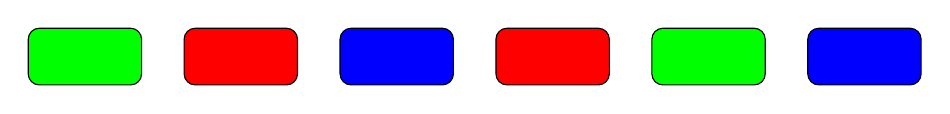
\begin{tikzpicture}[scale=.9]
\draw[rounded corners,fill=green] (0,0)  
  rectangle +(1.6cm,.8cm);
\draw[rounded corners,fill=red]   (2.2,0)
  rectangle +(1.6cm,.8cm);
\draw[rounded corners,fill=blue]  (4.4,0)
  rectangle +(1.6cm,.8cm);
\draw[rounded corners,fill=red]   (6.6,0)
  rectangle +(1.6cm,.8cm);
\draw[rounded corners,fill=green] (8.8,0)
  rectangle +(1.6cm,.8cm);
\draw[rounded corners,fill=blue]  (11,0)
  rectangle +(1.6cm,.8cm);
\end{tikzpicture}
\end{center}
\caption{Anordnung der Blöcke für das Langford-Problem}\label{f.langford}
\end{figure}

\begin{definition}[Langford-Problem $L(n)$] Gegeben sei die Menge\footnote{Ein \emph{multiset} oder \emph{bag} ist wie eine Menge, mit der Ausnahme, dass es mehr als ein Vorkommen eines Elements geben kann.} von positiven ganzen Zahlen:
\[
\{1,1,2,2,3,3,\ldots,n,n\}\,,
\]
Lassen sie sich so anordnen, dass für $1\leq i \leq n$ $i$ Zahlen zwischen den beiden Vorkommen von $i$ liegen?
\end{definition}

Abbildung~\ref{f.langford} zeigt, dass 312132 eine Lösung für $L(3)$ ist.

\smallskip

Abschnitt~\ref{s.langford-covering} formuliert das Langford-Problem neu und verwendet dabei einen mathematischen Formalismus, der die Lösung des Problems erleichtert. Abschnitt~\ref{s.langford-theorem} charakterisiert Werte von $n$, für die $L(n)$ lösbar ist, und präsentiert zwei Beweise des Satzes. Der erste Beweis, der relativ einfach ist, verwendet die Technik der Doppelzählung: man zählt denselben Wert auf zwei verschiedene Arten und setzt die resultierenden Formeln gleich. Der zweite Beweis ist eine geschickte Induktion, aber die damit verbundene ``Buchführung'' erfordert eine sorgfältige Beachtung der Details. Abschnitt~\ref{s.langford-four} arbeitet die Lösung für $L(4)$ aus.

\section(Langfords Problem als Deckungsproblem)\label{s.langford-covering}

Das Langford-Problem kann mit Hilfe einer Matrix gelöst werden. Für $L(3)$ gibt es sechs Spalten, eine für jede Position, an der die sechs Zahlen platziert werden können. Es gibt eine Zeile für jede mögliche Platzierung einer der Zahlen, d.h. die beiden Vorkommen von $k$ müssen $k$ Zahlen zwischen sich haben. Es gibt vier mögliche Platzierungen der $1$-Zahlen, drei der $2$-Zahlen und zwei der $3$-Zahlen:

\begin{center}
\addtolength{\tabcolsep}{4pt}
\begin{tabular}{|c||c|c|c|c|c|c|}
\hline
&1&2&3&4&5&6\\\hline\hline
1&1&&1&&&\\\hline
2&&1&&1&&\\\hline
3&&&1&&1&\\\hline
4&&&&1&&1\\\hline
5&2&&&2&&\\\hline
6&&2&&&2&\\\hline
7&&&2&&&2\\\hline
8&3&&&&3&\\\hline
9&&3&&&&3\\\hline
\end{tabular}
\end{center}
Um das Problem zu lösen, müssen wir eine Zeile für die $1$-Zahlen in der Folge, eine Zeile für die $2$-Zahlen und eine Zeile für die $3$-Zahlen auswählen, so dass, wenn wir diese Zeilen übereinander stapeln, keine Spalte mehr als eine Zahl enthält.

Die Zeile 9 braucht wegen der Symmetrie nicht berücksichtigt zu werden: Wenn man mit Zeile 9 beginnt, erhält man die Umkehrung der Folge, die man erhält, wenn man mit Zeile 8 beginnt.

Zeile 8 ist die einzige, die $3$ enthält, also muss sie gewählt werden, und die Folge ist 3\textvisiblespace \textvisiblespace \textvisiblespace 3\textvisiblespace. Jede Zeile mit Zahlen in den Spalten 1 und 5 kann nicht mehr verwendet werden, da an jeder Stelle nur eine Zahl stehen kann. Bezeichnen wir die zulässigen und verbotenen Zeilen mit:
\[\not\! 1,2,\not\! 3,4,\not\! 5, \not\! 6, 7, 8\,.\]

Zeile 7 ist die einzige verbleibende Zeile, die $2$'s enthält, also muss sie ausgewählt werden und die Reihenfolge ist 3\textvisiblespace 2\textvisiblespace 3{}2. Das Löschen von Zeilen, die nicht mehr verwendet werden können, ergibt:
\[\not\! 1,2,\not\! 3,\not\! 4,\not\! 5, \not\! 6, 7, 8\,.\]

Wählt man die einzige verbleibende Zeile, Zeile 2, ergibt sich die Lösung 3{}1{}2{}1{}3{}2:
\begin{center}
\addtolength{\tabcolsep}{4pt}
\begin{tabular}{|c||c|c|c|c|c|c|}
\hline
&1&2&3&4&5&6\\\hline\hline
2&&1&&1&&\\\hline
7&&&2&&&2\\\hline
8&3&&&&3&\\\hline
\end{tabular}
\end{center}
Die Analyse hat gezeigt, dass dies die einzige Lösung ist, mit Ausnahme der symmetrischen Lösung, die man erhält, wenn man mit Zeile 9 beginnt.

\section{Für welche Werte von $N$ ist das Langfordsche Problem lösbar?}\label{s.langford-theorem}

\begin{theorem} \label{thm.langford}
$L(n)$ hat dann und nur dann eine Lösung, wenn $n=4k$ oder $n=4k+3$.
\end{theorem}

Wir beweisen die Vorwärtsrichtung des Satzes. Beweis~1 zeigt, dass wenn $L(n)$ eine Lösung hat, dann $n=4k$ oder $n=4k+3$. Beweis~2 zeigt den Kehrsatz: wenn $n=4k+1$ oder $n=4k+2$, dann hat $L(n)$ keine Lösung.

\begin{proof}
(1) Wenn das erste Vorkommen der Zahl $k$ an der Stelle $i_k$ ist, ist das zweite Vorkommen an der Stelle $i_k+k+1$. Zum Beispiel in 3{}1{}2{}1{}3{}2, der Lösung für $L(3)$, ergibt die Wahl von $k=2$ $i_k=3$ und $i_k+k+1=3+2+1=6$.

$S_n$, die Summe der Positionen aller Zahlen, ist:
\begin{eqnarray*}
S_n&=&\sum_{k=1}^{n}i_k+\sum_{k=1}^{n}(i_k+k+1)\\
& =& 2\sum_{k=1}^{n}i_k+\sum_{k=1}^{n}(k+1)\\
&=& 2\sum_{k=1}^{n}i_k+\frac{n(n+3)}{2}\,.
\end{eqnarray*}
Aber $S_n$ ist einfach $1+2+3+\cdots+2n$, also:
\[
S_n=\sum_{k=1}^{2n}k = \frac{2n(2n+1)}{2}\,.
\]
Die Gleichsetzung der beiden Formeln für $S_n$ ergibt:
\begin{eqnarray*}
2\sum_{k=1}^{n}i_k+\frac{n(n+3)}{2} &=& \frac{2n(2n+1)}{2}\\
\sum_{k=1}^{n}i_k &=& \frac{1}{2}\left(\frac{2n(2n+1)}{2} - \frac{n(n+3)}{2}\right) \\
&=& \frac{3n^2-n}{4}\,.
\end{eqnarray*}

Die linke Seite ist eine ganze Zahl, da sie die Summe von ganzen Zahlen ist (die Positionen), also muss die rechte Seite auch eine ganze Zahl sein. Wann ist $3n^3-n$ durch $4$ teilbar? Die Faktorisierung von $3n^2-n$ ergibt $n(3n-1)$.

Wenn $n$ ein Vielfaches von $4$ ist, ist das Produkt durch $4$ teilbar.

Wann ist $3n-1$ durch $4$ teilbar? Jede ganze Zahl $n$ lässt sich als $n=4i+j$ für $j=0,1,2,3$ darstellen. Wenn $3n-1$ durch $4$ teilbar ist, dann ist auch $3(4i+j)-1 = 12i+3j-1$ teilbar. $12i$ ist durch $4$ teilbar. Für $j=\{0,1,2,3\}$ ist $3j-1=\{-1,2,5,8\}$ dann und nur dann durch $4$ teilbar, wenn $j=3$, also $n=4i+3$.
\end{proof}
Um die Idee des zweiten Beweises vorzustellen, betrachten wir, wie eine Lösung für $n=4$ aussehen könnte. In den folgenden Tabellen sind die Stellen, an denen 4 vorkommt, 1 und 6, und die Stellen, an denen 2 vorkommt, sind 5 und 8. In beiden Fällen ist eine Position ungerade und die andere gerade. 
\[
\begin{array}{|c|c|c|c|c|c|c|c|}
\hline
1&2&3&4&5&6&7&8\\
\hline\hline
4&1&3&1&2&4&3&2\\\hline
*&&&&&*&&\\\hline
\end{array}
\hspace{3em}
\begin{array}{|c|c|c|c|c|c|c|c|}
\hline
1&2&3&4&5&6&7&8\\
\hline\hline
4&1&3&1&2&4&3&2\\\hline
&&&&*&&&*\\\hline
\end{array}
\]
Sei $k=2m$ eine \emph{gerade} Zahl. Wenn $i$ die Position des ersten Vorkommens von $k$ ist, dann ist die Position des zweiten Vorkommens $i+k+1$.
Die Summe der Positionen ist:
\[
i+(i+k+1)=2i+2m+1=2(i+m)+1\,,
\]
was eine ungerade Zahl ist. Damit die Summe von zwei Zahlen ungerade ist, muss eine ungerade und die andere gerade sein.

Überprüfen wir nun die Positionen des Auftretens der ungeraden Zahlen. Die Positionen der Vorkommen von 1 sind 2 und 4, beides gerade Zahlen, und die Positionen der Vorkommen von 3 sind 3 und 7, beides ungerade Zahlen.
\[
\begin{array}{|c|c|c|c|c|c|c|c|}
\hline
1&2&3&4&5&6&7&8\\
\hline\hline
4&1&3&1&2&4&3&2\\\hline
&*&&*&&&&\\\hline
\end{array}
\hspace{3em}
\begin{array}{|c|c|c|c|c|c|c|c|}
\hline
1&2&3&4&5&6&7&8\\
\hline\hline
4&1&3&1&2&4&3&2\\\hline
&&*&&&&*&\\\hline
\end{array}
\]
Sei $k=2m+1$ eine \emph{odd} Zahl. Die Summe der Positionen ist:
\[
i+(i+k+1)=2i+2m+1+1=2(i+m+1)\,,
\]
was eine gerade Zahl ist. Damit die Summe von zwei Zahlen gerade ist, müssen beide ungerade oder beide gerade sein.

Die Positionen $1,2,\ldots,2n-1,2n$ enthalten eine gleiche Anzahl von geraden und ungeraden Positionen. Die beiden Vorkommen einer Zahl in einer Zeile ``bedecken'' zwei Stellen. Wenn die Menge der Zeilen alle Positionen abdeckt, müssen sie eine gleiche Anzahl von geraden und ungeraden Positionen abdecken. Definieren Sie die Parität einer Reihe von Zeilen als die Differenz zwischen der Anzahl der geraden und ungeraden Positionen, die abgedeckt werden. Zu Beginn ist die Parität gleich Null, und wenn das Problem eine Lösung hat, hat die Menge der Zeilen in der Lösung ebenfalls die Parität Null.

Wenn zwei Vorkommen einer geraden Zahl platziert werden, decken sie eine gerade und eine ungerade Position ab, so dass die Parität gleich bleibt:
\[
\begin{array}{|c|c|c|c|c|c|c|c|}
\hline
1&2&3&4&5&6&7&8\\
\hline\hline
4&1&3&1&2&4&3&2\\\hline
-1&&&&&+1&&\\\hline
\end{array}
\hspace{3em}
\begin{array}{|c|c|c|c|c|c|c|c|}
\hline
1&2&3&4&5&6&7&8\\
\hline\hline
4&1&3&1&2&4&3&2\\\hline
&&&&-1&&&+1\\\hline
\end{array}
\]
Wenn zwei Vorkommen einer ungeraden Zahl platziert werden, wird die Parität $+2$ oder $-2$, also müssen wir in der Lage sein, dieses Paar mit einem Paar von Vorkommen einer anderen ungeraden Zahl zu verbinden, die an Positionen platziert sind, die die Parität ausgleichen:
\[
\begin{array}{|c|c|c|c|c|c|c|c|}
\hline
1&2&3&4&5&6&7&8\\
\hline\hline
4&1&3&1&2&4&3&2\\\hline
&+1&&+1&&&&\\\hline
\end{array}
\hspace{3em}
\begin{array}{|c|c|c|c|c|c|c|c|}
\hline
1&2&3&4&5&6&7&8\\
\hline\hline
4&1&3&1&2&4&3&2\\\hline
&&-1&&&&-1&\\\hline
\end{array}
\]
Wir haben gezeigt, dass es eine Lösung des Langford-Problems nur dann geben kann, wenn es eine gerade Anzahl ungerader Zahlen in $\{1,\ldots,n\}$ gibt!
Das Theorem besagt, dass, wenn dies wahr ist, entweder $n=4k$ oder $n=4k-1$, und wenn nicht, dann entweder $n=4k-2$ oder $4k-3$.

\begin{proof}
(2)
Der Beweis erfolgt durch Induktion.
Es gibt vier Grundfälle:
\begin{itemize}
\item $n=4k-3=1$. In $\{1\}$ gibt es eine ungerade Anzahl von ungeraden Zahlen und es gibt keine Lösung.
\item $n=4k-2=2$. In $\{1,2\}$ gibt es eine ungerade Anzahl von ungeraden Zahlen und es gibt keine Lösung.
\item $n=4k-1=3$. In $\{1,2,3\}$ gibt es eine gerade Anzahl von ungeraden Zahlen und wir haben gesehen, dass es eine Lösung gibt.
\item $n=4k-0$. In $\{1,2,3,4\}$ gibt es eine gerade Anzahl von ungeraden Zahlen und Sect.~\ref{s.langford-four} gibt eine Lösung.
\end{itemize}

Die induktive Hypothese ist, dass der Satz für $\{1,\ldots,4k-j\}$, $k\ge 1$, $0\leq j\leq 3$ wahr ist, und wir werden beweisen, dass er für $n=4(k+1)-j$ wahr ist.

\begin{itemize}
\item Füge $4k+1=4(k+1)-3$ zu $\{1,\ldots,4k\}$ hinzu. Nach der Induktionshypothese für $4k=4k-0$ gibt es eine gerade Anzahl von ungeraden Zahlen. $4(k+1)-3$ ist ungerade, also gibt es jetzt eine ungerade Anzahl von ungeraden Zahlen und es gibt keine Lösung.
\item Füge $4k+2=4(k+1)-2$ zu $\{1,\ldots,4k+1\}$ hinzu. Nach der Induktionshypothese für $4k+1=4(k+1)-3$ gibt es eine ungerade Anzahl von ungeraden Zahlen. $4(k+1)-2$ ist gerade, also gibt es immer noch eine ungerade Anzahl von ungeraden Zahlen und es gibt keine Lösung.
\item Füge $4k+3=4(k+1)-1$ zu $\{1,\ldots,4k+2\}$ hinzu. Nach der Induktionshypothese für $4k+2=4(k+1)-2$ gibt es eine ungerade Anzahl von ungeraden Zahlen. $4(k+1)-1$ ist ungerade, also gibt es eine gerade Anzahl von ungeraden Zahlen und es gibt wahrscheinlich eine Lösung.
\item Füge $4k+4=4(k+1)-0$ zu $\{1,2,\ldots,4k+3\}$ hinzu. Nach der Induktionshypothese für $4k+3=4(k+1)-1$ gibt es eine gerade Anzahl von ungeraden Zahlen. $4(k+1)-0$ ist gerade, also gibt es eine gerade Anzahl von ungeraden Zahlen und eine Lösung ist wahrscheinlich.
\end{itemize}
\end{proof}

%%%%%%%%%%%% Solution for L(4) %%%%%%%%%%%%%%%%%%

\newpage

\section{Lösung für $L(4)$}\label{s.langford-four}


Hier ist das Feld für $L(4)$. Versuchen Sie, die Lösung selbst zu finden.
\begin{center}
\addtolength{\tabcolsep}{4pt}
\begin{tabular}{|c||c|c|c|c|c|c|c|c|}
\hline
&1&2&3&4&5&6&7&8\\\hline\hline
1&1&&1&&&&&\\\hline
2&&1&&1&&&&\\\hline
3&&&1&&1&&&\\\hline
4&&&&1&&1&&\\\hline
5&&&&&1&&1&\\\hline
6&&&&&&1&&1\\\hline
7&2&&&2&&&&\\\hline
8&&2&&&2&&&\\\hline
9&&&2&&&2&&\\\hline
10&&&&2&&&2&\\\hline
11&&&&&2&&&2\\\hline
12&3&&&&3&&&\\\hline
13&&3&&&&3&&\\\hline
14&&&3&&&&3&\\\hline
15&&&&3&&&&3\\\hline
16&4&&&&&4&&\\\hline
17&&4&&&&&4&\\\hline
18&&&4&&&&&4\\\hline
\end{tabular}
\end{center}
Aus Gründen der Symmetrie kann die Zeile 18 entfallen.

\smallskip

%$1,2,3,4,5,6,7,8,9,10,11,12,13,14,15,16,17$
\noindent Wählen Sie Zeile 16 und die Reihenfolge ist 4\textvisiblespace\textvisiblespace\textvisiblespace\textvisiblespace 4 \textvisiblespace\textvisiblespace.
Jede Zeile mit einem Element an Position $1$ oder Position $6$ kann nicht mehr Teil der Lösung sein.

$\not\! 1,2,3,\not\! 4,5,\not\! 6,\not\! 7,8,\not\! 9,10,11,\not\!\! 12,\not\!\! 13,14,15,16,\not\!\! 17$

\noindent Wählen Sie Zeile 14 und die Reihenfolge ist 4\textvisiblespace 3\textvisiblespace\textvisiblespace 4{}3\textvisiblespace.

$\not\! 1,2,\not\! 3,\not\! 4,\not\! 5,\not\! 6,\not\! 7,8,\not\! 9,\not\!\! 10,11,\not\!\! 12,\not\!\! 13,14, \not\!\! 15,16,\not\!\! 17$

\noindent Wählen Sie Zeile 8. Die Reihenfolge ist 4{}2{}3\textvisiblespace 2{}4{}3\textvisiblespace.

$\not\! 1,\not\! 2,\not\! 3,\not\! 4,\not\! 5,\not\! 6,\not\! 7,8,\not\! 9,\not\!\! 10,\not\!\! 11,\not\!\! 12,\not\!\! 13,14, \not\!\! 15,16,\not\!\! 17$

\noindent Alle Auswahlmöglichkeiten für die 1 wurden eliminiert, also müssen wir zurückgehen.

\smallskip

\noindent Anstelle von Zeile 8 wählen Sie Zeile 11 und die Reihenfolge ist 4\textvisiblespace 3\textvisiblespace 2{}4{}3{}2.


$\not\! 1,2,\not\! 3,\not\! 4,\not\! 5,\not\! 6,\not\! 7,\not\! 8,\not\! 9,\not\!\! 10,11,\not\!\! 12,\not\!\! 13,14, \not\!\! 15,16,\not\!\! 17$

\noindent Wählen Sie Zeile 2 und wir haben eine Lösung 4{}1{}3{}1{}2{}4{}3{}2.

\smallskip

\noindent Gehen Sie weiter zurück, um zu sehen, ob es eine andere Lösung gibt.

\smallskip

\noindent Anstelle von Zeile 14 wählen Sie Zeile 15 und die Reihenfolge ist 4\textvisiblespace \textvisiblespace 3\textvisiblespace 4\textvisiblespace 3.

$\not\! 1,\not\! 2,3,\not\! 4,5,\not\! 6,\not\! 7,8,\not\! 9,\not\!\! 10,\not\!\! 11,\not\!\! 12,\not\!\! 13,\not\!\! 14,15,16,\not\!\! 17$

\noindent Reihe 8 muss gewählt werden und die Reihenfolge ist 4{}2\textvisiblespace 3{}2{}4\textvisiblespace 3.

$\not\! 1,\not\! 2,\not\! 3,\not\! 4,\not\! 5,\not\! 6,\not\! 7,8,\not\! 9,\not\!\! 10,\not\!\! 11,\not\!\! 12,\not\!\! 13,\not\!\! 14,15,16,\not\!\! 17$

\noindent Alle Möglichkeiten für die 1 wurden gestrichen, also gehen wir wieder zurück.

\smallskip

\noindent Anstelle von Zeile 16 wählen Sie Zeile 17 und die Reihenfolge ist \textvisiblespace 4\textvisiblespace \textvisiblespace \textvisiblespace\textvisiblespace 4\textvisiblespace.

$1,\not\! 2,3,4,\not\! 5,6,7,\not\! 8,9,\not\!\! 10,11,12,\not\!\! 13,\not\!\! 14,15,\not\!\! 16,17$

\noindent Wählen Sie Zeile 15 und die Reihenfolge ist \textvisiblespace 4\textvisiblespace 3\textvisiblespace\textvisiblespace 4{}3.

$1,\not\! 2,3,\not\! 4,\not\! 5,\not\! 6,\not\! 7,\not\! 8,9,\not\!\! 10,\not\!\! 11,\not\!\! 12,\not\!\! 13,\not\!\! 14,15,\not\!\! 16,17$

\noindent Reihe 9 muss gewählt werden und die Reihenfolge ist \textvisiblespace 4{}2{}3\textvisiblespace 2{}4{}3.

$1,\not\! 2,\not\! 3,\not\! 4,\not\! 5,\not\! 6,\not\! 7,\not\! 8,9,\not\!\! 10,\not\!\! 11,\not\!\! 12,\not\!\! 13,\not\!\! 14,15,\not\!\! 16,17$

\noindent Alle Auswahlmöglichkeiten für die 1 wurden eliminiert. Wir können ein letztes Mal zurückgehen. 
%$1,\not\! 2,3,4,\not\! 5,6,7,\not\! 8,9,\not\! 10,11,12,\not\! 13,\not\! 14,15,\not\! 16,17$

\smallskip

\noindent Anstelle von Reihe 15 wählen Sie Reihe 12 und die Folge ist 3{}4\textvisiblespace \textvisiblespace 3\textvisiblespace 4.

$\not\! 1,\not\! 2,\not\! 3,\not\! 4,\not\! 5,\not\! 6,\not\! 7,\not\! 8,9,\not\!\! 10,\not\!\! 11,12,\not\!\! 13,\not\!\! 14,\not\!\! 15,\not\!\! 16,17$

\noindent Auch hier wurden alle Möglichkeiten für die 1er gestrichen.

\medskip

\noindent Daher ist die einzige Lösung $41312432$.

\subsection*{Was ist die Überraschung?}

Die Quelle der Inspiration für ein mathematisches Theorem kann überraschend sein. Langford bemerkte ein Muster in den farbigen Blöcken seines Sohnes, das zu dem interessanten Thm.~\ref{thm.langford} führte. Die Schüler sollten auch erfahren, dass ein Satz viele verschiedene Beweise haben kann.

\subsection*{Quellen}
Dieses Kapitel stützt sich auf \cite{miller}. \cite{davies} zeigt, wie man eine Lösung für $n=4k$ und $n=4k+3$ findet.
